\documentclass{report}
\usepackage{Sweave}
\usepackage{graphicx}
\usepackage[francais]{babel} 
\usepackage[utf8]{inputenc}
\usepackage[T1]{fontenc} 
\usepackage{amsmath} 
\usepackage{amsfonts}
\usepackage{verbatim} 
\usepackage{float} 
\usepackage{hyperref}
\usepackage{scrtime}

\begin{document}
\input{GAL-Buckle95-concordance}

\title{GAL Buckle 95}
\author{François Pelletier}
\maketitle
\tableofcontents

\chapter{Initialisation}

\section{Chargement des paquets}
\begin{Schunk}
\begin{Sinput}
> setwd("~/git/GAL-Buckle95/")
> library(actuar)
> library(MASS)
> library(xtable)
> library(multicore)
> library(moments)
> library(TTR)
> library(FourierStuff)
> library(GeneralizedAsymmetricLaplace)
> library(GMMStuff)
> library(OptionPricingStuff)
> library(QuadraticEstimatingEquations)
\end{Sinput}
\end{Schunk}

\section{Constantes et données}

\begin{Schunk}
\begin{Sinput}
> #Nombre de décimales affichées
> options(digits=6)
> #Marge pour intervalles de confiance
> alpha.confint <- 0.05 
> #Marge pour test d'hypothèses
> alpha.test <- 0.05
> #Chargement des données
> RETURNS <- head(read.csv("abbeyn.csv",sep="\t",header=TRUE)[,1],-1)
> #Taille de l'échantillon
> n <- length(RETURNS)
\end{Sinput}
\end{Schunk}

\section{Test de normalité}

\begin{Schunk}
\begin{Sinput}
> EppsPulley.test(RETURNS)
\end{Sinput}
\begin{Soutput}
Epps-Pulley Normality test

 T: 0.626033
 T*: 0.635568
p-value: 0.007178

$Tstat
[1] 0.626033

$Tmod
[1] 0.635568

$Zscore
[1] 2.44824

$Pvalue
[1] 0.00717788

$Reject
[1] TRUE
\end{Soutput}
\end{Schunk}

\chapter{Estimation}

\section{Données mises à l'échelle}

\begin{Schunk}
\begin{Sinput}
> sRET <- as.vector(scale(RETURNS))
\end{Sinput}
\end{Schunk}

\section{Première estimation par QEE}

\begin{Schunk}
\begin{Sinput}
> ## Point de départ	
> pt.depart <- startparamGAL(sRET)
> ## Fonctions pour les moments
> meanQEE <- function(param) mGAL(param,1)
> varianceQEE <- function(param) cmGAL(param,2)
> sdQEE <- function(param) sqrt(cmGAL(param,2))
> skewnessQEE <- function(param) cmGAL(param,3)
> kurtosisQEE <- function(param) cmGAL(param,4)
> ## Fonctions pour les dérivées
> dmeanQEE <- function(param) dmGAL(param,1)
> dsdQEE <- function(param) dmGAL(param,2)
> ## Estimation gaussienne
> optim1 <- optim(pt.depart,obj.gauss,gr=NULL,sRET,
+ 		meanQEE,varianceQEE,dmeanQEE,dsdQEE)
> pt.optim1 <- optim1$par
> ## Estimation de crowder
> optim2 <- optim(pt.depart,obj.Crowder,gr=NULL,sRET,
+ 		meanQEE,varianceQEE,skewnessQEE,kurtosisQEE,dmeanQEE,dsdQEE)
> pt.optim2 <- optim2$par
> ## Estimation de crowder modifiée
> optim3 <- optim(pt.depart,obj.Crowder.Mod,gr=NULL,sRET,
+ 		meanQEE,varianceQEE,dmeanQEE,dsdQEE)
> pt.optim3 <- optim3$par
\end{Sinput}
\end{Schunk}

\section{Résultats de la première estimation par QEE}

\begin{Schunk}
\begin{Sinput}
> cov.optim1 <- covariance.QEE(M.gauss(pt.optim1,sRET,
+ 				meanQEE,varianceQEE,dmeanQEE,dsdQEE),
+ 		V.gauss(pt.optim1,sRET,meanQEE,varianceQEE,
+ 				skewnessQEE,kurtosisQEE,dmeanQEE,dsdQEE),n)
> cov.optim2 <- covariance.QEE(M.Crowder(pt.optim2,sRET,
+ 				varianceQEE,skewnessQEE,kurtosisQEE,dmeanQEE,dsdQEE),
+ 		V.Crowder(pt.optim2,sRET,varianceQEE,
+ 				skewnessQEE,kurtosisQEE,dmeanQEE,dsdQEE),n)
> cov.optim3 <- covariance.QEE(M.Crowder.Mod(pt.optim3,sRET,
+ 				varianceQEE,skewnessQEE,kurtosisQEE,dmeanQEE,dsdQEE),
+ 		V.Crowder.Mod(pt.optim3,sRET,varianceQEE,dmeanQEE,dsdQEE),n)
> confidence.interval.QEE(pt.optim1,cov.optim1,n)
\end{Sinput}
\begin{Soutput}
         LOWER  ESTIMATE     UPPER
[1,] -0.780018 -0.726048 -0.672077
[2,]  0.436002  0.596316  0.756630
[3,]  0.262650  0.359186  0.455722
[4,]  1.994757  2.021370  2.047982
\end{Soutput}
\begin{Sinput}
> confidence.interval.QEE(pt.optim2,cov.optim2,n)
\end{Sinput}
\begin{Soutput}
         LOWER  ESTIMATE     UPPER
[1,] -0.694457 -0.627404 -0.560351
[2,]  0.413764  0.640292  0.866820
[3,]  0.232650  0.334028  0.435405
[4,]  1.839966  1.878296  1.916626
\end{Soutput}
\begin{Sinput}
> confidence.interval.QEE(pt.optim3,cov.optim3,n)
\end{Sinput}
\begin{Soutput}
         LOWER  ESTIMATE     UPPER
[1,] -0.765288 -0.711439 -0.657589
[2,]  0.455485  0.606642  0.757798
[3,]  0.264669  0.362932  0.461195
[4,]  1.932691  1.960299  1.987906
\end{Soutput}
\end{Schunk}

\section{Seconde estimation par QEE}

\begin{Schunk}
\begin{Sinput}
> ## Estimation gaussienne
> optim4 <- optim(pt.optim1,obj.gauss,gr=NULL,sRET,
+ 		meanQEE,varianceQEE,dmeanQEE,dsdQEE,
+ 		ginv(V.gauss(pt.optim1,sRET,meanQEE,
+ 						varianceQEE,skewnessQEE,kurtosisQEE,
+ 						dmeanQEE,dsdQEE)))
> pt.optim4 <- optim4$par
> ## Estimation de crowder
> optim5 <- optim(pt.optim2,obj.Crowder,gr=NULL,sRET,
+ 		meanQEE,varianceQEE,skewnessQEE,kurtosisQEE,dmeanQEE,dsdQEE,
+ 		ginv(V.Crowder(pt.optim2,sRET,varianceQEE,skewnessQEE,
+ 						kurtosisQEE,dmeanQEE,dsdQEE)))
> pt.optim5 <- optim5$par
> ## Estimation de crowder modifiée
> optim6 <- optim(pt.optim3,obj.Crowder.Mod,gr=NULL,sRET,
+ 		meanQEE,varianceQEE,dmeanQEE,dsdQEE,
+ 		ginv(V.Crowder.Mod(pt.optim3,sRET,varianceQEE,
+ 						dmeanQEE,dsdQEE)))
> pt.optim6 <- optim6$par
\end{Sinput}
\end{Schunk}

\section{Résultats de la seconde estimation par QEE}

\begin{Schunk}
\begin{Sinput}
> cov.optim4 <- covariance.QEE(M.gauss(pt.optim4,sRET,
+ 				meanQEE,varianceQEE,dmeanQEE,dsdQEE),
+ 		V.gauss(pt.optim4,sRET,meanQEE,varianceQEE,
+ 				skewnessQEE,kurtosisQEE,dmeanQEE,dsdQEE),n)
> cov.optim5 <- covariance.QEE(M.Crowder(pt.optim5,sRET,
+ 				varianceQEE,skewnessQEE,kurtosisQEE,dmeanQEE,dsdQEE),
+ 		V.Crowder(pt.optim5,sRET,varianceQEE,skewnessQEE,
+ 				kurtosisQEE,dmeanQEE,dsdQEE),n)
> cov.optim6 <- covariance.QEE(M.Crowder.Mod(pt.optim6,sRET,
+ 				varianceQEE,skewnessQEE,kurtosisQEE,dmeanQEE,dsdQEE),
+ 		V.Crowder.Mod(pt.optim6,sRET,varianceQEE,dmeanQEE,dsdQEE),n)
> confidence.interval.QEE(pt.optim4,cov.optim4,n)
\end{Sinput}
\begin{Soutput}
         LOWER  ESTIMATE     UPPER
[1,] -0.779792 -0.725853 -0.671914
[2,]  0.436017  0.596319  0.756622
[3,]  0.262456  0.358969  0.455482
[4,]  1.995452  2.022048  2.048644
\end{Soutput}
\begin{Sinput}
> confidence.interval.QEE(pt.optim5,cov.optim5,n)
\end{Sinput}
\begin{Soutput}
         LOWER  ESTIMATE     UPPER
[1,] -0.692712 -0.625874 -0.559036
[2,]  0.414139  0.640445  0.866750
[3,]  0.231568  0.332845  0.434122
[4,]  1.842116  1.880376  1.918636
\end{Soutput}
\begin{Sinput}
> confidence.interval.QEE(pt.optim6,cov.optim6,n)
\end{Sinput}
\begin{Soutput}
         LOWER  ESTIMATE     UPPER
[1,] -0.766288 -0.712450 -0.658612
[2,]  0.455051  0.606193  0.757334
[3,]  0.264972  0.363196  0.461419
[4,]  1.934050  1.961614  1.989178
\end{Soutput}
\end{Schunk}

\section{Estimation par GMM}

\begin{Schunk}
\begin{Sinput}
> ## GMM régulier
> optim7 <- optim.GMM(pt.depart,
+ 		conditions.vector=meanvariance.gmm.vector,
+ 		data=sRET,W=diag(2),
+ 		meanf=meanQEE,variancef=varianceQEE)
> pt.optim7 <- optim7$par
> cov.optim7 <- mean.variance.GMM.gradient.GAL(pt.optim7,sRET) %*% 
+ 		covariance.GMM(meanvariance.gmm.vector,pt.optim7,sRET,
+ 				meanf=meanQEE,variancef=varianceQEE) %*%
+ 		t(mean.variance.GMM.gradient.GAL(pt.optim7,sRET)) / n
> ## GMM itératif
> optim8 <- iterative.GMM(pt.depart,
+ 		conditions.vector=meanvariance.gmm.vector,
+ 		data=sRET,W=diag(2),
+ 		meanf=meanQEE,variancef=varianceQEE)
> pt.optim8 <- optim8$par
> cov.optim8 <-  mean.variance.GMM.gradient.GAL(pt.optim8,sRET) %*% 
+ 		optim8$cov %*%  
+ 		t(mean.variance.GMM.gradient.GAL(pt.optim8,sRET)) / n
> confidence.interval.QEE(pt.optim7,cov.optim7,n)
\end{Sinput}
\begin{Soutput}
         LOWER  ESTIMATE     UPPER
[1,] -0.878702 -0.641646 -0.404589
[2,] -0.469225  0.625908  1.721040
[3,] -0.192234  0.326366  0.844965
[4,]  1.696121  1.965995  2.235869
\end{Soutput}
\begin{Sinput}
> confidence.interval.QEE(pt.optim8,cov.optim8,n)
\end{Sinput}
\begin{Soutput}
         LOWER  ESTIMATE     UPPER
[1,] -0.874031 -0.636980 -0.399929
[2,] -0.473292  0.626346  1.725984
[3,] -0.193600  0.322895  0.839390
[4,]  1.704166  1.972716  2.241265
\end{Soutput}
\end{Schunk}

\chapter{Comparaison des résultats}
\begin{Schunk}
\begin{Sinput}
> # Aggrégation des estimateurs (pour simplifier les calculs)
> pts.estim <- cbind(pt.optim1,pt.optim2,pt.optim3,pt.optim4,
+ 		pt.optim5,pt.optim6,pt.optim7,pt.optim8)
> l.pts.estim <- as.list(data.frame(pts.estim))
\end{Sinput}
\end{Schunk}

\section{Fonction de répartition}
\begin{Schunk}
\begin{Sinput}
> # Points d'évaluation
> xi <- seq(2*min(sRET),2*max(sRET),length.out=2^6)
> # Fonction de répartition par intégration de la fonction caractéristique
> dist1 <- cbind(cftocdf(xi,cfGAL,param=pt.optim1),
+ 		cftocdf(xi,cfGAL,param=pt.optim2),
+ 		cftocdf(xi,cfGAL,param=pt.optim3),
+ 		cftocdf(xi,cfGAL,param=pt.optim4),
+ 		cftocdf(xi,cfGAL,param=pt.optim5),
+ 		cftocdf(xi,cfGAL,param=pt.optim6),
+ 		cftocdf(xi,cfGAL,param=pt.optim7),
+ 		cftocdf(xi,cfGAL,param=pt.optim8))
> # Fonction de répartition par point de selle
> dist2 <- cbind(psaddleapproxGAL(xi,pt.optim1),
+ 		psaddleapproxGAL(xi,pt.optim2),
+ 		psaddleapproxGAL(xi,pt.optim3),
+ 		psaddleapproxGAL(xi,pt.optim4),
+ 		psaddleapproxGAL(xi,pt.optim5),
+ 		psaddleapproxGAL(xi,pt.optim6),
+ 		psaddleapproxGAL(xi,pt.optim7),
+ 		psaddleapproxGAL(xi,pt.optim8))
> # Fonction de répartition par intégration de la fonction de densité
> dist3 <- cbind(pGAL(xi,pt.optim1),
+ 		pGAL(xi,pt.optim2),
+ 		pGAL(xi,pt.optim3),
+ 		pGAL(xi,pt.optim4),
+ 		pGAL(xi,pt.optim5),
+ 		pGAL(xi,pt.optim6),
+ 		pGAL(xi,pt.optim7),
+ 		pGAL(xi,pt.optim8))
\end{Sinput}
\end{Schunk}
\pagebreak
\subsection{Graphiques}

\begin{Schunk}
\begin{Sinput}
> 	for (i in 1:8)
+ 	{
+ 		file<-paste("dist-GAL-",i,".pdf",sep="")
+ 		pdf(file=file,paper="special",width=6,height=6)
+ 		plot.ecdf(sRET,main=paste("Fonction de répartition ",i))
+ 		lines(xi,dist1[,i],col="green")
+ 		lines(xi,dist2[,1],col="red")
+ 		lines(xi,dist3[,1],col="pink")
+ 		lines(xi,pnorm(xi),type="l",col="blue")
+ 		dev.off()
+ 		cat("\\includegraphics[height=2in,width=2in]{",
+ 				file,"}\n",sep="")
+ 	}
\end{Sinput}
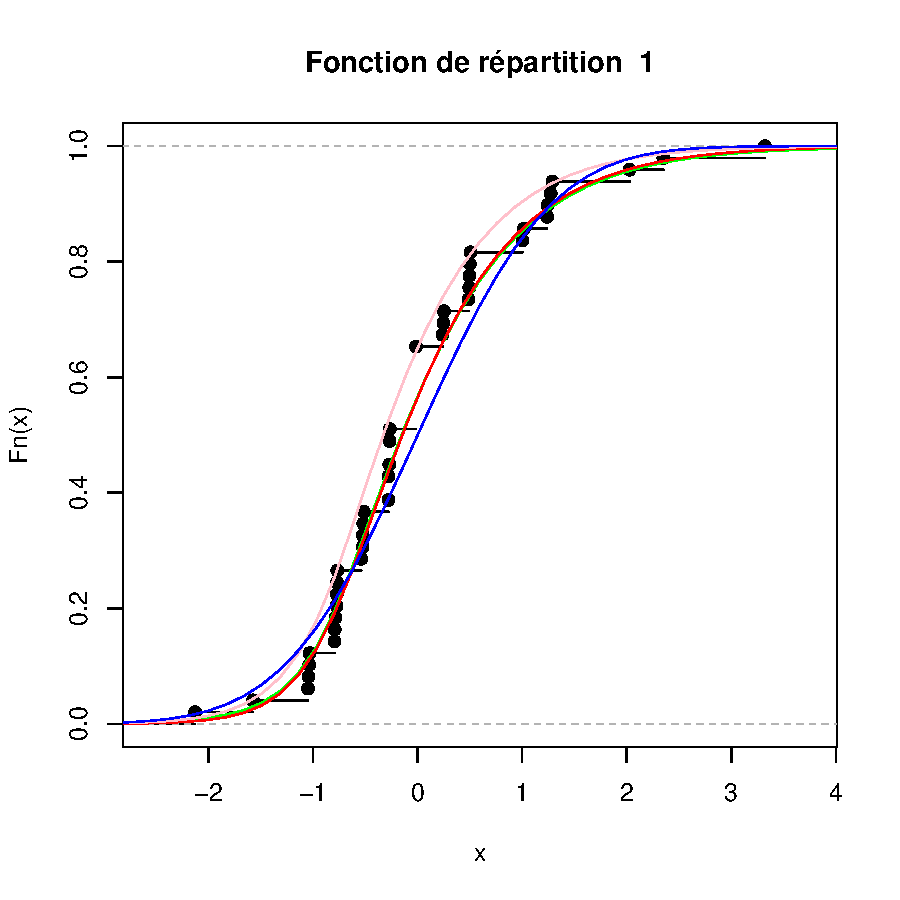
\includegraphics[height=2in,width=2in]{dist-GAL-1.pdf}
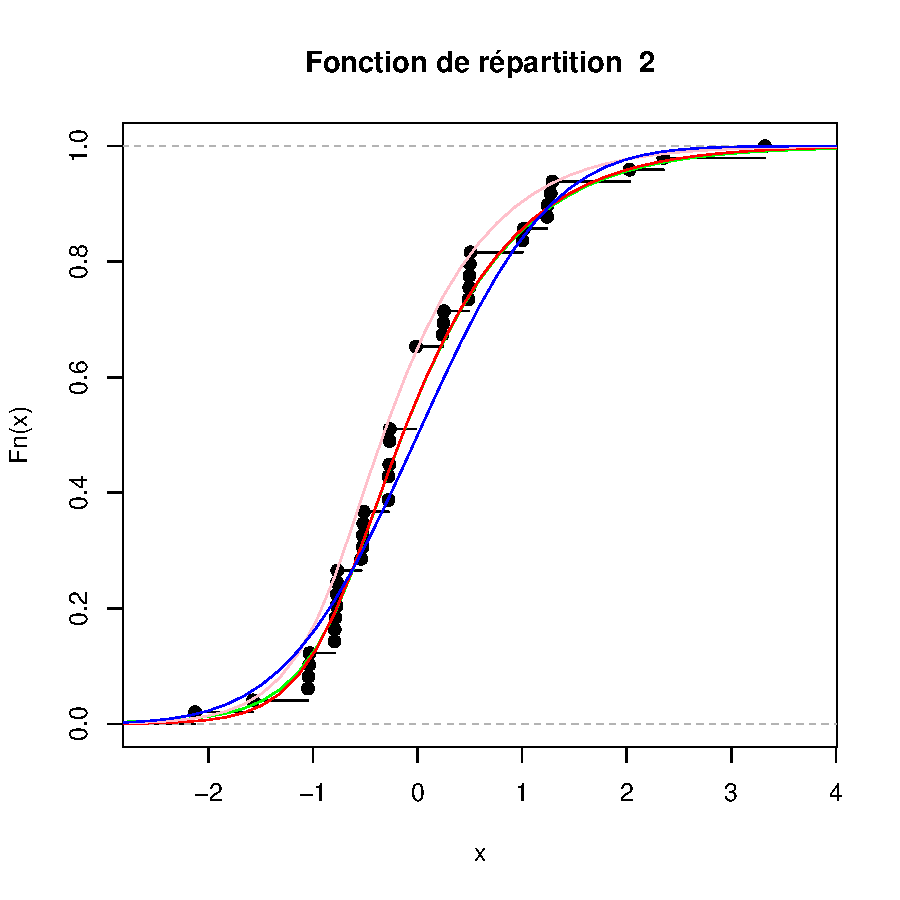
\includegraphics[height=2in,width=2in]{dist-GAL-2.pdf}
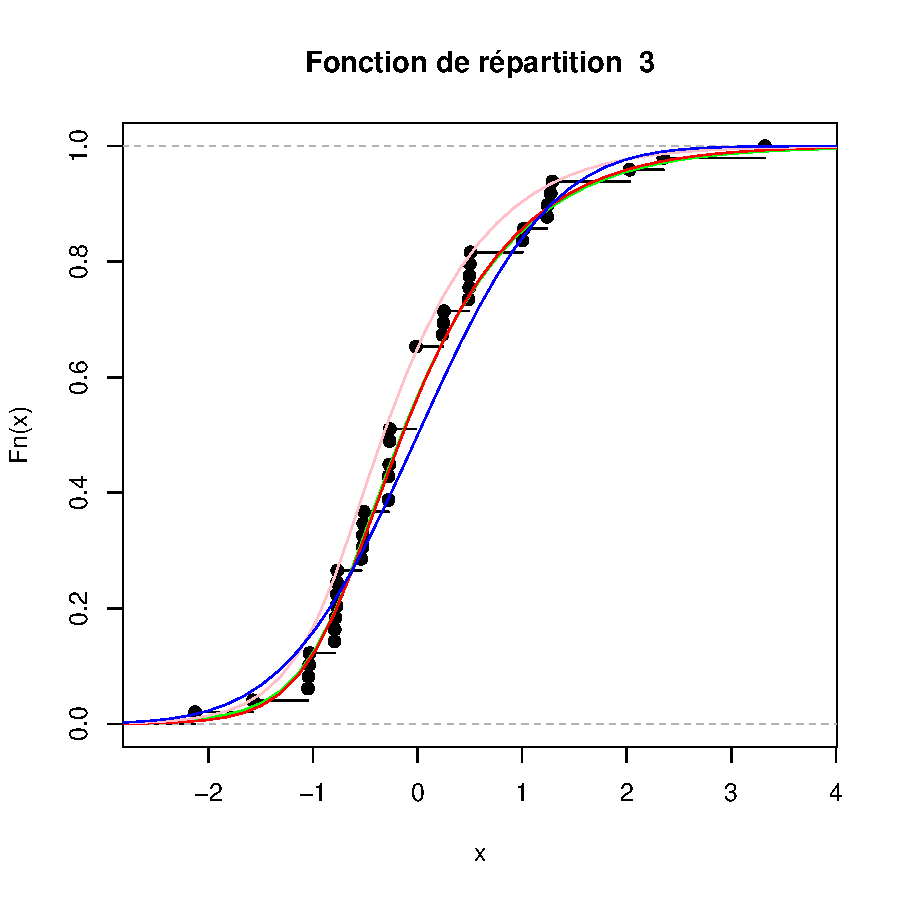
\includegraphics[height=2in,width=2in]{dist-GAL-3.pdf}
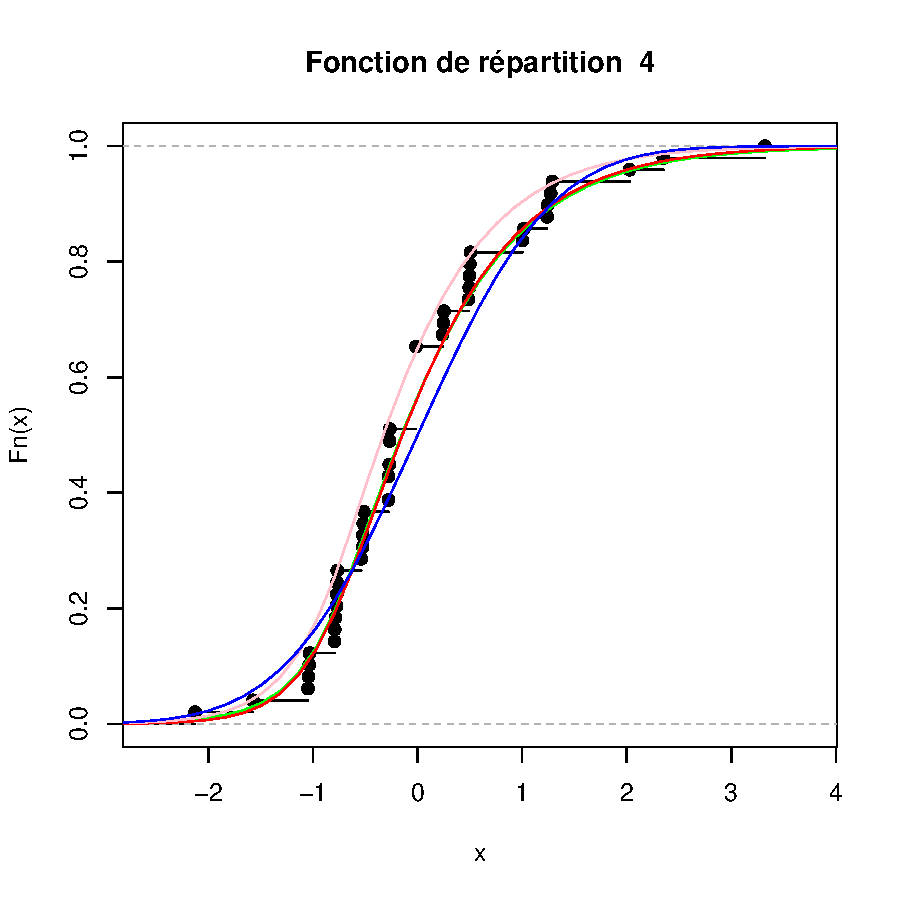
\includegraphics[height=2in,width=2in]{dist-GAL-4.pdf}
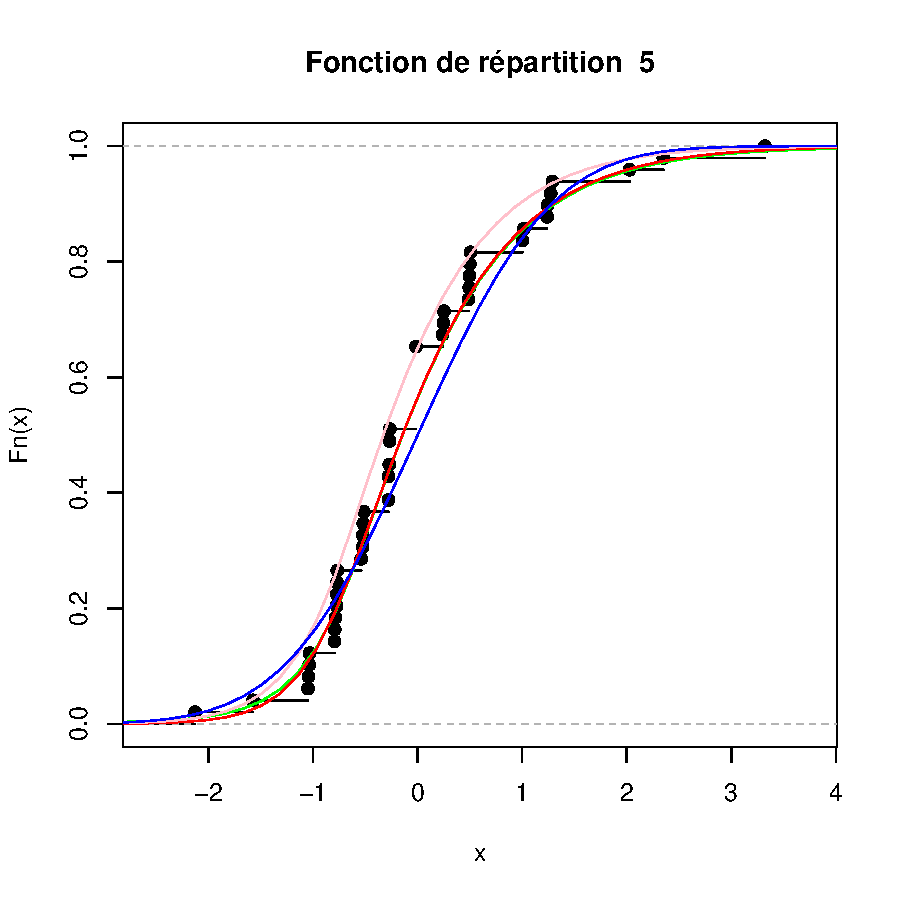
\includegraphics[height=2in,width=2in]{dist-GAL-5.pdf}
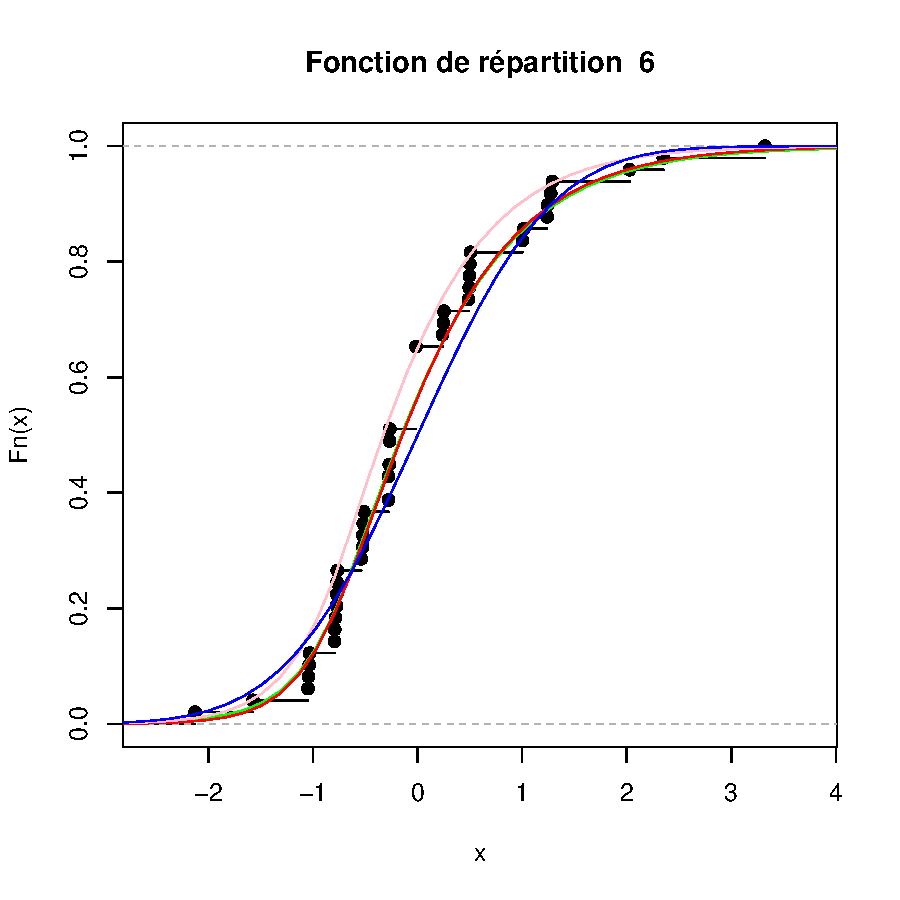
\includegraphics[height=2in,width=2in]{dist-GAL-6.pdf}
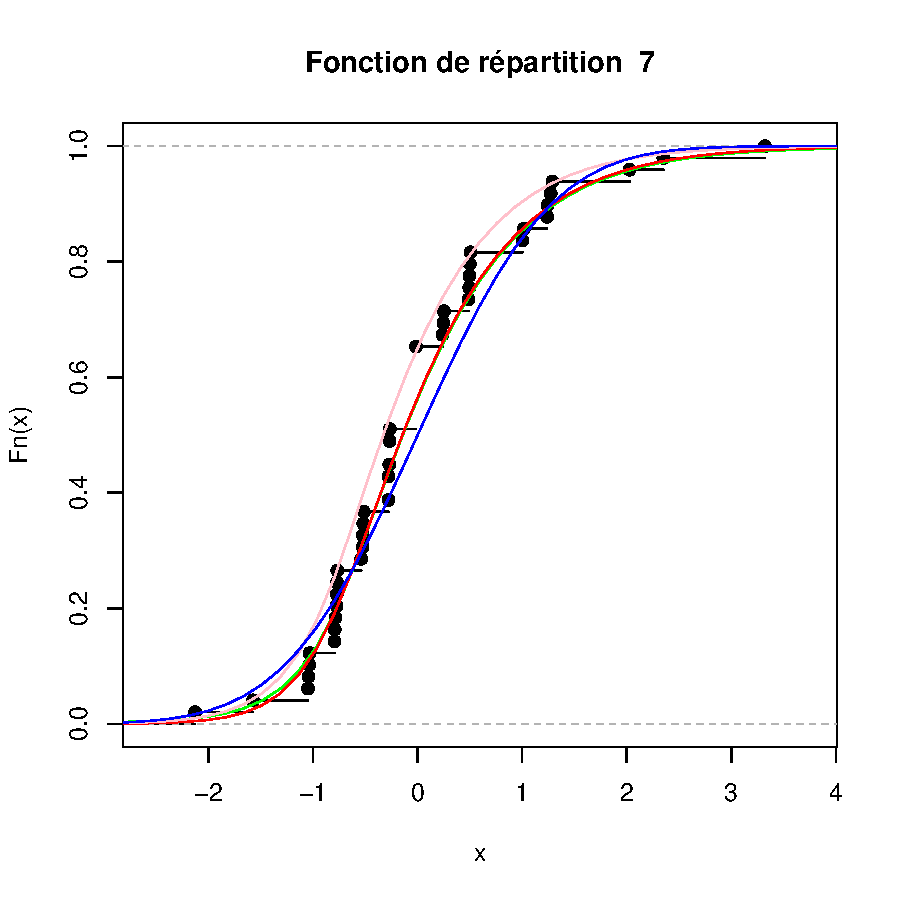
\includegraphics[height=2in,width=2in]{dist-GAL-7.pdf}
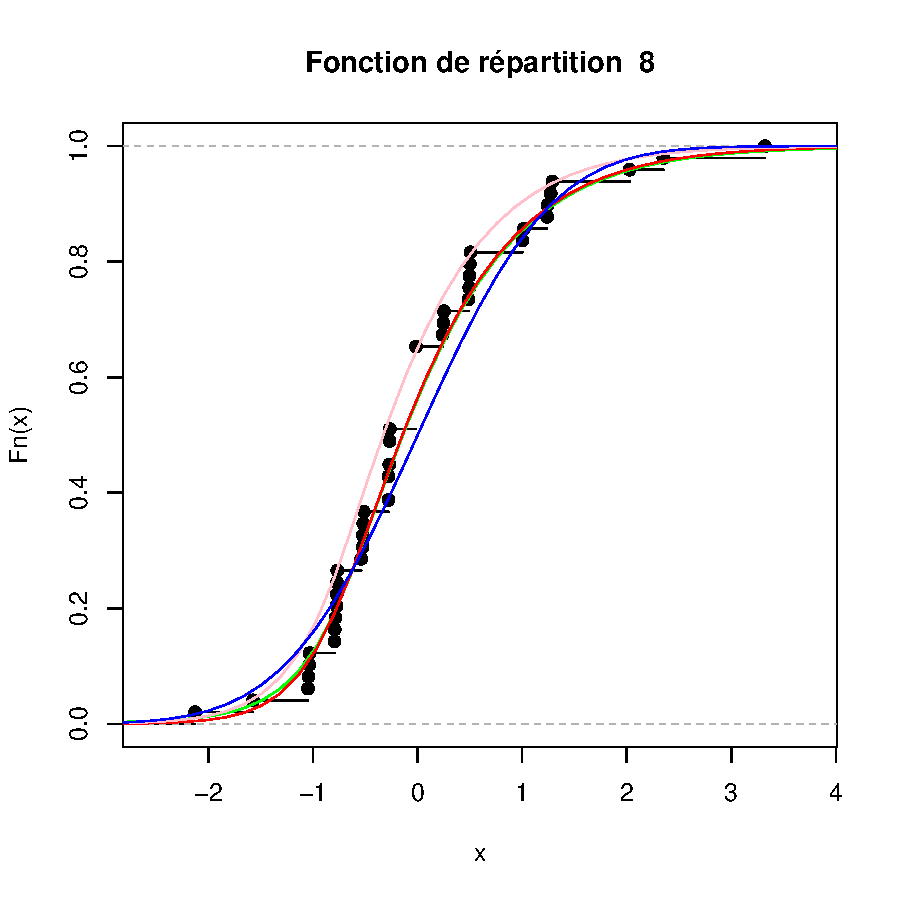
\includegraphics[height=2in,width=2in]{dist-GAL-8.pdf}\end{Schunk}

\subsection{Statistiques}
Test du $\chi^2$, Méthode avec intégration
\begin{Schunk}
\begin{Sinput}
> chisquare.test1 <- function(param,DATA.hist,FUN,method)
+ {
+ 	chisquare.test(DATA.hist,FUN,param,method=method)
+ }
> xtable(do.call(rbind,lapply(l.pts.estim,chisquare.test1,hist(sRET),cfGAL,"integral")),digits=6)
\end{Sinput}
% latex table generated in R 3.0.2 by xtable 1.7-1 package
% Sat Mar 15 11:38:58 2014
\begin{table}[ht]
\centering
\begin{tabular}{rrrr}
  \hline
 & chisquare.stat & df & p.value \\ 
  \hline
pt.optim1 & 5.473824 & 6.000000 & 0.484626 \\ 
  pt.optim2 & 5.329673 & 6.000000 & 0.502277 \\ 
  pt.optim3 & 5.388158 & 6.000000 & 0.495076 \\ 
  pt.optim4 & 5.474310 & 6.000000 & 0.484567 \\ 
  pt.optim5 & 5.337004 & 6.000000 & 0.501372 \\ 
  pt.optim6 & 5.390662 & 6.000000 & 0.494769 \\ 
  pt.optim7 & 5.454256 & 6.000000 & 0.487003 \\ 
  pt.optim8 & 5.476963 & 6.000000 & 0.484245 \\ 
   \hline
\end{tabular}
\end{table}\end{Schunk}

Test du $\chi^2$, Méthode avec point de selle
\begin{Schunk}
\begin{Sinput}
> xtable(do.call(rbind,lapply(l.pts.estim,chisquare.test1,hist(sRET),pGAL,"saddlepoint")),digits=6)
\end{Sinput}
% latex table generated in R 3.0.2 by xtable 1.7-1 package
% Sat Mar 15 11:38:58 2014
\begin{table}[ht]
\centering
\begin{tabular}{rrrr}
  \hline
 & chisquare.stat & df & p.value \\ 
  \hline
pt.optim1 & 9.293574 & 6.000000 & 0.157728 \\ 
  pt.optim2 & 8.345592 & 6.000000 & 0.213862 \\ 
  pt.optim3 & 9.050625 & 6.000000 & 0.170751 \\ 
  pt.optim4 & 9.292836 & 6.000000 & 0.157767 \\ 
  pt.optim5 & 8.344140 & 6.000000 & 0.213959 \\ 
  pt.optim6 & 9.062381 & 6.000000 & 0.170100 \\ 
  pt.optim7 & 8.616379 & 6.000000 & 0.196330 \\ 
  pt.optim8 & 8.610490 & 6.000000 & 0.196698 \\ 
   \hline
\end{tabular}
\end{table}\end{Schunk}

Statistique de Kolmogorov-Smirnov
\begin{Schunk}
\begin{Sinput}
> 	ks.test1 <- function(param,x,y) ks.test(x,y,param)
> 	xtable(do.call(rbind,mclapply(l.pts.estim,ks.test1,sRET,"pGAL")),digits=6)
\end{Sinput}
% latex table generated in R 3.0.2 by xtable 1.7-1 package
% Sat Mar 15 11:38:58 2014
\begin{table}[ht]
\centering
\begin{tabular}{rrrrrr}
  \hline
 & statistic & p.value & alternative & method & data.name \\ 
  \hline
pt.optim1 & 0.158220 & 0.171912 & two-sided & One-sample Kolmogorov-Smirnov test & x \\ 
  pt.optim2 & 0.140346 & 0.289345 & two-sided & One-sample Kolmogorov-Smirnov test & x \\ 
  pt.optim3 & 0.156772 & 0.179751 & two-sided & One-sample Kolmogorov-Smirnov test & x \\ 
  pt.optim4 & 0.158159 & 0.172235 & two-sided & One-sample Kolmogorov-Smirnov test & x \\ 
  pt.optim5 & 0.139916 & 0.292753 & two-sided & One-sample Kolmogorov-Smirnov test & x \\ 
  pt.optim6 & 0.156960 & 0.178718 & two-sided & One-sample Kolmogorov-Smirnov test & x \\ 
  pt.optim7 & 0.141230 & 0.282437 & two-sided & One-sample Kolmogorov-Smirnov test & x \\ 
  pt.optim8 & 0.140016 & 0.291954 & two-sided & One-sample Kolmogorov-Smirnov test & x \\ 
   \hline
\end{tabular}
\end{table}\end{Schunk}

Statistique de distance minimale

\begin{Schunk}
\begin{Sinput}
> 	tvariate1 <- seq(-.1,.1,by=0.01)
> 	xtable(do.call(rbind,mclapply(l.pts.estim,md.test,sRET,tvariate1,cfGAL,empCF)),digits=6)
\end{Sinput}
% latex table generated in R 3.0.2 by xtable 1.7-1 package
% Sat Mar 15 11:38:58 2014
\begin{table}[ht]
\centering
\begin{tabular}{rrrr}
  \hline
 & md.stat & df & p.value \\ 
  \hline
pt.optim1 & 0.000422 & 21.000000 & 0.000000 \\ 
  pt.optim2 & 0.120174 & 21.000000 & 0.000000 \\ 
  pt.optim3 & 0.001384 & 21.000000 & 0.000000 \\ 
  pt.optim4 & 0.000388 & 21.000000 & 0.000000 \\ 
  pt.optim5 & 0.123295 & 21.000000 & 0.000000 \\ 
  pt.optim6 & 0.001451 & 21.000000 & 0.000000 \\ 
  pt.optim7 & 0.007980 & 21.000000 & 0.000000 \\ 
  pt.optim8 & 0.010416 & 21.000000 & 0.000000 \\ 
   \hline
\end{tabular}
\end{table}\end{Schunk}






\end{document}
